\documentclass[border=2pt]{standalone}
\usepackage[dvipsnames,svgnames,x11names]{xcolor}
\usepackage{tikz}
\usetikzlibrary{arrows.meta,shapes.geometric}
\begin{document}
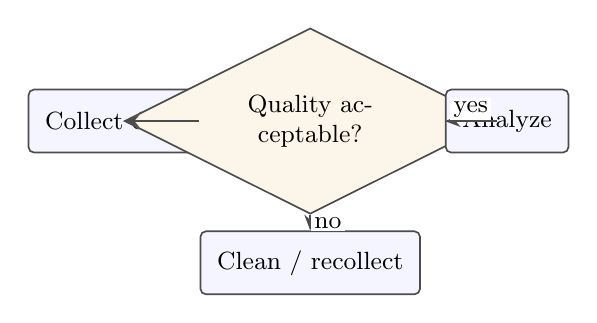
\begin{tikzpicture}[font=\small,>=Stealth,x=25mm,y=18mm]
\node[rectangle,rounded corners=2pt,fill=blue!4,draw=black!70,text=black,line width=0.6pt,minimum height=8mm,inner xsep=6pt,inner ysep=4pt,align=center] (start) at (0,0) {Collect data};
\node[diamond,aspect=2,fill=Goldenrod!10,draw=black!70,text=black,line width=0.6pt,minimum height=8mm,inner xsep=6pt,inner ysep=4pt,align=center,text width=24mm] (check) at (1,0) {Quality acceptable?};
\node[rectangle,rounded corners=2pt,fill=blue!4,draw=black!70,text=black,line width=0.6pt,minimum height=8mm,inner xsep=6pt,inner ysep=4pt,align=center] (accept) at (2,0) {Analyze};
\node[rectangle,rounded corners=2pt,fill=blue!4,draw=black!70,text=black,line width=0.6pt,minimum height=8mm,inner xsep=6pt,inner ysep=4pt,align=center] (reject) at (1,-1) {Clean / recollect};
\draw[->,draw=black!70,line width=0.6pt] (start) -- (check);
\draw[->,draw=black!70,line width=0.6pt] (check) -- node[pos=0.5,above,fill=white,inner sep=1.2pt] {yes} (accept);
\draw[->,draw=black!70,line width=0.6pt] (check) -- node[pos=0.5,right,fill=white,inner sep=1.2pt] {no} (reject);
\end{tikzpicture}
\end{document}
